\chapter{Related Work}

This chapter follows by mentioning related work regarding the current implementation of the C\# compiler and formalizing C\# type inference using Hindley-Milner type inference, which is explored in more detail with references to its modification in Rust and C\# programming languages.
This knowledge will be utilized as a primary source of inspiration for the improvement.
In the end, it mentions relevant C\# language issues presented on the GitHub repository, which will be used later to prioritize the improvement features to make it more likely to be discussed at Language Design Meetings (LDM) held by Language Design Team (LDT). 

\section{Roslyn} \label{sect04:roslyn}

The implementation of C\# type inference can be found in the Roslyn compiler, as open-source C\# and VisualBasic compiler developed at the GitHub repository \cite{online:roslynRepo}. 
Presented Roslyn’s architecture will help to better understand the context and restrictions that has to be cosidered to plug the improved type inference into the compiler.
Figure \ref{img15:roslynPip} is used to explain the compilation pipeline \cite{online:roslynArchitecture} which consists of four phases highlighted with different colors.
\begin{figure}[h]
\centering
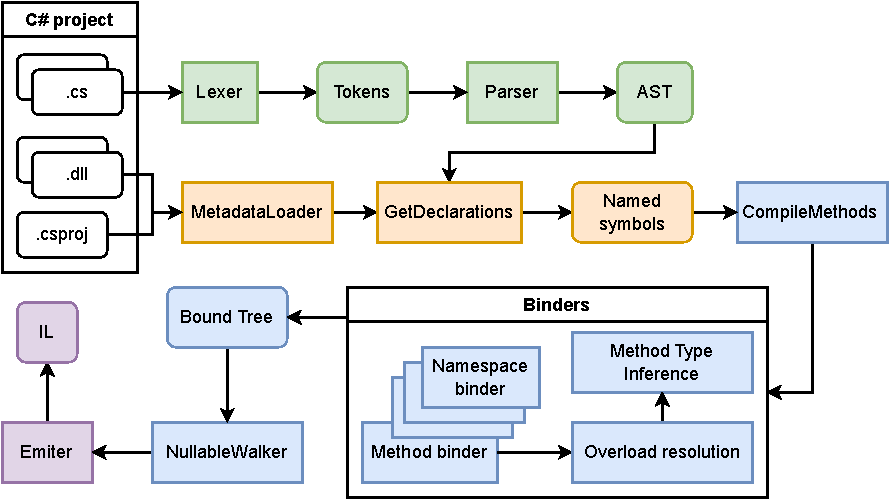
\includegraphics[width=140mm]{./img/Roslyn.pdf}
\caption{Roslyn architecture}
\label{img15:roslynPip}
\end{figure}

\subsection{Parsing C\# Sources Phase}

The pipeline starts with loading the \texttt{.csproj} file with related C\# sources (\texttt{.cs}) and referenced libraries (\texttt{.dll}).
C\# sources are passed to the lexer, creating tokens used by the parser forming Abstract Syntax Tree (AST).
AST construction is the first phase (green boxes in Figure \ref{img15:roslynPip}) of the compiler checking the syntax of C\# sources.

\subsection{Loading Named Symbols}

The second phase, marked by orange, forms \emph{named symbols} exposed by public API representing defined namespaces, classes, methods, etc., in the C\# project. 
The declarations are received from C\# sources by traversing AST and seeking for the particular syntax. 
Libraries, stored in the \texttt{.dll} format are parsed by \texttt{MetadataLoader}, creating the same named symbols as those received from C\# sources.

\subsection{Binding Phase}

The third phase (represented by blue boxes), also called the binding phase, matches identifiers in the code with received named symbols from the previous phase. 
Because the processing of a method body is not dependent on other method bodies since the code only uses already known declarations, Roslyn makes this phase concurrent. 
The result of the phase is a \emph{bound tree} where all identifiers refer to the named symbols. 
A method binding itself is a complicated procedure consisting of many subtasks such as \emph{overload resolution} or mentioned method type inference, whose algorithm is described in detail in the previous section \ref{sect02:MTIA}.
\par
The binding is divided into a chain of binders, taking care of smaller code scopes. 
One purpose of the binders is the ability to resolve an identifier to the named symbol if the referred symbol lies in their scope. 
If they can’t find the symbol, they ask the preceding binder. 
The process of finding referred symbols is called \emph{LookUp}. 
Examples of binders are \texttt{NamespaceBinder} resolving defined top-level entities in the namespace scope, \texttt{ClassBinder} resolving defined class members, or \texttt{MethodBinder} binding method bodies. 
The last mentioned binder sequentially iterates body statements and matches identifiers with their declarations. 
The statement and expression binding are important steps that are related to type inference.
An important observation is that statement binding doesn’t involve binding of the following statements, which can be referred to as backward binding. 
The consequence is that C\# is not able to infer types in the backward direction. 
An example can be the usage of the \texttt{var} keyword in variable declarations, which has to be used always with the initializing value. 
If C\# would allow backward binding, we could initialize the variable later in one of the following statements which would determine the type of the variable.
\par
The preceding step before method type inference is overload resolution, part of \texttt{MethodCallExpression} or \texttt{ObjectCreationExpression} binding. 
As mentioned previously, method overloading allows to define multiple methods with the same name differing in parameters. 
So, when the compiler decides which method should be called, it has to resolve the right version of the method by following language rules for the method resolution. 
This step involves binding the method call arguments first and then deciding which parameter list of the method group fits the argument list the best. 
If the method group is generic and the expression doesn’t specify any type arguments, the method type inference is invoked to determine the type arguments of the method before the selection of the best candidate for the call.
When the right overload with inferred type arguments is chosen, unbound method arguments requiring the target type (for example already mentioned the target-typed \texttt{new()} operator) are bound using the corresponding parameter type.
\par
The method type inference can occur for the second time if the previously mentioned nullability analysis is turned on. 
The nullability analysis is a kind of a flow analysis that uses a bound tree to check and rewrite already created bound nodes according to nullability. 
Because overloading and the method type inference are nullable-sensitive, the whole binding process is repeated, respecting the nullability and reusing results from the previous binding. 
The required changes are stored during the analysis, and the Bound tree is rewritten by the changes at the end of the analysis.

\subsection{Emiting Code Phase}

The last phase, marked by purple, emits Common Intermediate Language (CIL) code targeting the .NET virtual machine.
The code is later loaded and executed by .NET runtime.

\section{Hindley-Millner Type Inference} \label{sect03:HM}

C\# method type inference is a restricted Hindley-Millner type inference which is able to work in C\# type system.
Since type inference in other languages like Rust or Haskell is based on the same principle, a high-level overview of Hindley-Millner type inference is presented together with its type system to formalize the C\# type inference, compare it with Rust type inference formalization and propose possible extensions of current C\# type inference based on these observations.
\par
Hindley-Millner type system \cite{online:wikiHM} is a type system for \textit{lambda calculus} capable of generic functions and types.
Lambda calculus contains four types of expressions given below which are described in the video series \cite{online:HMVideos} regarding Hindley-Millner type inference explanation.
An expression is either a variable (\ref{expr01}), a function application (\ref{expr02}), a lambda function (\ref{expr03}), or a \textit{let-in} clause (\ref{expr04}).
\begin{align}
e =&\ x\label{expr01}\\
|&\ e_1 e_2\label{expr02}\\
|&\ \lambda x \rightarrow e\label{expr03}\\
|&\ \text{\textbf{let}}\ x = e_1\ \text{\textbf{in}}\ e_2\label{expr04} 
\end{align}
\par
The above-mentioned expressions have one of two kinds of types.
The \textit{Mono} type is a type variable(\ref{type01}) or a function application(\ref{type02}) where \textit{C} is an item from an arbitrary set of functions containing at least the \texttt{$\rightarrow$} symbol taking two type parameters which represents a lambda function type.
The second kind is the \textit{Poly} type, which is an arbitrary type with possible preceding the $\forall$ operator \ref{type04}, bounding its type variables.
\par
\begin{align}
mono\ \tau =&\ \alpha\label{type01}\\
|&\ C\ \tau_1,...,\tau_n\label{type02}\\
poly\ \sigma =&\ \tau\label{type03}\\
|&\ \forall \alpha\ .\ \sigma\label{type04}
\end{align}
A context(represented by the \texttt{$\Gamma$} symbol) contains bindings of an expression to its type which are described by pairs of an expression and its type using the \texttt{$x:\tau$} syntax.
An assumption is than described as a typing judgment shown in the \texttt{$\Gamma$ $\vdash$ $x:\tau$} syntax meaning "In the given context \texttt{$\Gamma$}, \texttt{$x$} has the \texttt{$\tau$} type".
\par
The H-M deduction system gives the following inference rules, allowing to deduce the type of an expression based on the assumption given in the context. 
The syntax of a rule corresponds with what can be judged below the line based on assumptions given above the line.
The rules can be divided into two kinds.
The first four rules give a manual on what types can be expected by applying the mentioned expressions of lambda calculus. 
The two last rules allow to convert Poly types to Mono types and vice-versa.
\begin{align*}
\frac{x : \sigma \in \Gamma}{\Gamma \vdash x : \sigma}&[Variable]\\
\frac{\Gamma \vdash e_0 : \tau_a \rightarrow \tau_b\ \ \ \Gamma \vdash e_1 : \tau_a}{\Gamma \vdash e_0 e_1 : \tau_b}&[Function\ application]\\
\frac{\Gamma, x : \tau_a \vdash e : \tau_b}{\Gamma \vdash \lambda x \rightarrow e : \tau_a \rightarrow \tau_b}&[Function\ abstraction]\\
\frac{\Gamma \rightarrow e_0 : \sigma \ \ \ \Gamma , x : \sigma \vdash e_1 : \tau}{\Gamma \vdash\ \text{\textbf{let}}\ x = e_0\ \text{\textbf{in}}\ e_1 : \tau}&[Let\ clause]\\
\frac{\Gamma \vdash e : \sigma_a \ \ \ \sigma_a \sqsubseteq \sigma_b}{\Gamma \vdash e : \sigma_b}&[Instantiate]\\
\frac{\Gamma \vdash e : \sigma \ \ \ \alpha \notin Free(\Gamma)}{\Gamma \vdash e : \forall \alpha\ .\ \sigma}&[Generalize]\\
\end{align*}
\par
H-M type inference is able to find the type of every expression of a completely untyped program using only these type rules.
Although, there exist several algorithms for the inference Figure \ref{img16:w} shows only the W algorithm since it is closely related to C\# and Rust type inference.
Inputs are the context $\Gamma$ and an expression whose type has to be inferred.
The process consists of systematic traversing the expression from bottom to top and deducing the type of sub-expressions following the mentioned rules.
The algorithm contains the \texttt{Instantiate} method which replaces quantified type variables in the expression with new type variables, the \texttt{Generelize} method replacing free type variables in the expression with quantified type variables, and the \texttt{Unify} method, also known as \textit{unification} in \textit{logic}.
Unification is an algorithm finding a substitution of type variables whose application on the unifying types makes them identical. 
Outputs of this algorithm are the inferred type with a substitution used for the algorithm's internal state. 
\begin{figure}
\begin{lstlisting}[style=myAlgo, mathescape=true]
fn Infer($\Gamma$, expr):
  switch(expr):
    expr isLike 'x' $\rightarrow$ return ({}, Instantiate(expr))
    expr isLike '$\lambda x \rightarrow e$' $\rightarrow$
      $\beta$ = NewVar()
      ($S_1$, $\tau_1$) = Infer($\Gamma$ + x: $\beta$, e)
      return ($S_1$, $S_1$$\beta$ $\rightarrow$ $\tau_1$)
    expr isLike '$e_1$$e_2$' $\rightarrow$
      ($S_1$, $\tau_1$) = Infer($\Gamma$, $e_1$)
      ($S_2$, $\tau_2$) = Infer($S_1$$\Gamma$, $e_2$)
      $\beta$ = NewVar()
      ($S_3$, $\tau_1$) = Unify($S_2$$\tau_1$, $\tau_2$ $\rightarrow$ $\beta$)
      return ($S_3$$S_2$$S_1$, $S_3$$\beta$)
    expr isLike 'let x = $e_1$ in $e_2$' $\rightarrow$
      ($S_1$, $\tau_1$) = Infer($\Gamma$, $e_1$)
      ($S_2$, $\tau_2$) = Infer($\Gamma$ + x: Generalize($S_1$$\Gamma$, $\tau_1$), $e_2$)
      return ($S_2$$S_1$, $\tau_2$)
\end{lstlisting}
\caption{\textit{W} algorithm}
\label{img16:w}
\end{figure}
\par
We can notice that the unification part of this algorithm is similar to the method type inference mentioned in the C\# section \ref{sect02:MTIA} where the substitution represents inferred type arguments of the method whose parameter types were unified with corresponding argument types.
The same concept of the unification is also used in Rust type inference.

\newpage

\subsection{H-M Extensions}

H-M type system doesn't allow subtyping known from Rust or overloading known from C\#.  
\par
A basic principle of extending H-M type inference by subtyping is described in Parreaux's work \cite{paper:Parreaux}, where instead of accumulating type equivalent constraints, it accumulates and propagates subtyping constraints.
These subtyping constraints consist of a set of types, which have to be inherited by the constrained type variable, or the variable has to inherit them.
\par
Extending H-M type inference by supporting overloading is mentioned in Andreas Stadelmeier and Martin Plumicke's work \cite{paper:Overloading}.
An important thought behind this paper is to accumulate two types of type variable constraint sets.
Constraints observed from a method call are added into one \textit{AND-set}.
When the method call has multiple overloads, the AND-sets are added to the \textit{OR-set}.
After accumulating these sets, all combinations of items in OR-sets are generated and solved by type inference.
For each method overload participating in type inference, it makes an type inference containing constraints obtained only from the overloaded method, excluding constraints obtained from other overloads.
This algorithm can be improved by excluding overloads that can't be used in the method call to save the branching.
However, in the worst case, it still takes exponential time to infer types.

\section{Rust Type Inference}

Rust is a strongly typed programming language developed by Mozilla and an open community created for performance and memory safety without a garbage collection. 
Besides its specific features like traits or variable regions, it also has advanced type inference \cite{online:rustTypeInference}, which is now described in a high-level perspective to get an inspiration for the proposed C\# improvement.
\par
Figure \ref{img17:rustCodeExample} shows a significant difference between C\# type inference and global Rust type inference.
There is the \texttt{a} variable declaraction initialized by the \texttt{Vec<T>} generic type whose type argument is going to be inferred.
The second statement calls the \texttt{push} method on the \texttt{a} variable, which is also generic and takes an argument of the \texttt{T} type.
Since the \texttt{1} value is passed into this call, \texttt{T} is inferred to be the \texttt{i32} type and the type argument of the creating vector becomes \texttt{i32}.
An interesting behavior regarding the type inference is that it infers the type of creating object used in the first statement using information obtained from the second statement.
\begin{figure}[h]
\begin{lstlisting}
let mut a = Vec::new();
a.push(1);
\end{lstlisting}
\caption{Rust type inference example.}
\label{img17:rustCodeExample}
\end{figure}
\par
This global type inference is possible thanks to a type inference context which is shared across multiple statements. 
Figure \ref{img18:rustTypeInference} shows a basic principle of how the context is gradually filled by type variables' constraints deduced from the statements.   
As the compiler traverses a method body, it adds new type variables that have to be solved and constrains them by the types which they are interacting with. 
The figure demonstrates it by adding a new type variable \texttt{T1} representing a type of the \texttt{a} variable.
It uses the \texttt{sub} function which adds the \texttt{Vec<T2>} subtyping constaint to the \texttt{T1} variable represented by a thick green line.
This constraint was obtained from a type of the initializing value \texttt{Vec::new()} which contains an unspecified type argument represented by a new \texttt{T2} type variable.
Since, the initializing type can't be fully resolved because the constraint contains the \texttt{T2} unbound type variable it has to postpone the resolution.
\begin{figure}[h]
\centering
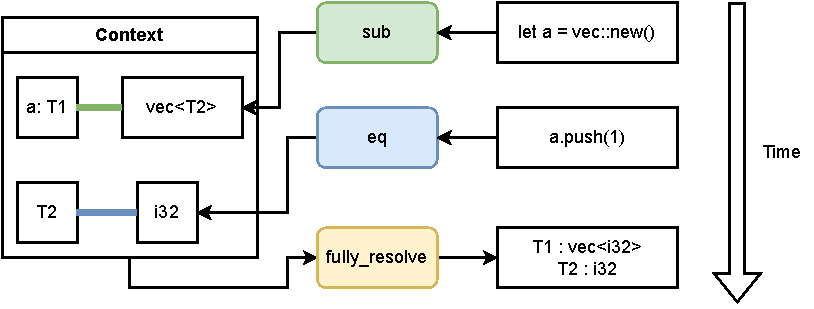
\includegraphics[width=140mm]{./img/RustTypeInference.pdf}
\caption{Rust type inference}
\label{img18:rustTypeInference}
\end{figure}
It passes the context to binding the next statement, where it collects another constraint about the \texttt{T2} type argument of the initializing value.
The \texttt{sub} function is similar to the unification seen in the previous section \ref{sect03:HM}, where it extracts the required bounds of unbound type variables by finding substitutions for type variables in order to make matching types containing the type variables equal.
When there is enough information to resolve \texttt{T1} and \texttt{T2} type variables, they are resolved by finding an appropriate type for the type variable with respect to collected bounds.
In the given example, the bounds contain only one type, so the type variables are resolved to them.
\par
The mentioned sharing of context enables type inference to be backward, meaning that based on future type information, it is possible to infer already collected unbounded type variables. 
Besides sharing the context, there are other inference features that are missing in C\# type inference and would be valuable. 
The first of them is type inference in object creation expressions, which doesn't exist in C\#. 
The next regards collecting type constraints, which are obtained from a wider context than C\# uses. 
For example, If a generic method containing a type variable in the return type is used as an assignment of an already typed variable, the type variable is constrained by the type of the target. Other features regard the implementation detail of type inference, which offers probing to constrain a type variable without influencing the context. 
There is a possibility of a snapshot that records all changes and can be used for backtracking and finding the right inferred type arguments.
Although Rust type inference is more advanced in comparison with C\#, it has to be considered language differences making type inference computation cost and difficulty relative to their features. 
As an example, the mentioned overloading can cause exponetial time of type inference. 
Since Rust doesn't have overloading, the type inference can be more powerful without significant slowdown, which is not the case of C\# as will be shown in the following chapters.

\section{Language Design GitHub Issues} \label{sect04:github}

Some ideas for type inference improvements have already been introduced in discussions in the C\# language repository \cite{online:langRepo}, which will be used as inspiration for the thesis’s proposed improvement.
However, before describing the related ideas, a process of proposing new C\# language features is mentioned to better understand how the ideas and final language changes are proceeded.

\subsection{Design Process and Championed Issue} \label{sect:champion}

The process of designing a new language feature starts with publishing an idea into discussions \cite{online:discussions}, where the C\# community can comment on it. 
The idea contains a brief description of the feature, motivation, and design. 
Besides the idea, a new language feature requires a proposal, initially published as an GitHub issue, describing the feature in a way that can be later reviewed by the LDM committee.
If the proposal sufficiently merits the discussions, it can be marked as a \textit{champion} by a member of LDT for being discussed further in LDM. 
The state of a proposal is described by several milestones. 
The most important for the thesis is the \textit{AnyTime} milestone, meaning that the proposal is not actively worked on and is open to the community to collaborate on it. 
At the time of writing, a member of LDT recommended a championed issue \cite{online:champion} regarding \textit{partial type inference} to be investigated since it contains many related discussions with proposed changes but still doesn’t have a required proposal specification which would allow to be discussed by the team. 
When a proposal has sufficient quality to be discussed by LDT, a member invites the proposer to make a \textit{pull request} where further collaboration continues. 
If LDT accepts the proposal, it is added to the \textit{proposals} folder in the repository for being added into the C\# specification, and its future implementation (in Roslyn) will be shipped with the next C\# version. 
\par
The recommended issue doesn't contain a specific idea of the improvemenet rather the scope of the improvement.
The improvement suggests \textit{partial type inference} which would allow to hint ambigious type arguments which can't be inferred by a compiler instead of currently specifying the whole type argument list.
Since it doesn't have any concerete way how to achive it, there are presented related discussion topics directly or indirectly mentioned in the issue which partially suggest a possible solution.

\subsection{Topic: Default Type Parameters} \label{sect07:is1}

One of the discussion \cite{online:DefTypeParam} mentions \textit{default type parameters} introducing default type arguments, which are used when explicit type arguments are not used. 
Figure \ref{img19:defTypeParam} shows a potential design of this feature where construing generic type \texttt{A} doesn’t need a type argument since it uses the \texttt{int} type as a default value. 
\begin{figure}[h]
\begin{lstlisting}[style=csharp]
class A<T = int> {}
...
var temp = new A();
\end{lstlisting}
\caption{Default type parameters.}
\label{img19:defTypeParam}
\end{figure}

\subsection{Topic: Generic Aliases} \label{sect08:is2}

Another discussion \cite{online:GenAlias} mentions \textit{generic aliases} allowing to specify default values similar to the goal of the previous discussion by defining an alias to that type with option generic parameters. 
Figure \ref{img20:genAlias} shows an example where there is the \texttt{StringDictionary} generic alias specifying the first type argument of the \texttt{Dictionary} class to be the \texttt{string} type, which simplifies the usage of the \texttt{Dictionary} type in scenarios where there are often used dictionaries with keys of the \texttt{string} type.
\begin{figure}[h]
\begin{lstlisting}[style=csharp]
using StringDictionary<TValue> = Dictionary<String, TValue>;
...
var temp = new StringDictionary<int>();
\end{lstlisting}
\caption{Generic aliases.}
\label{img20:genAlias}
\end{figure}

\subsection{Topic: Named Type Parameters} \label{sect09:is3}

The discussion \cite{online:NamedTypeParam} mentions \textit{named type parameters}, which are similar to named parameters of methods. 
The basic thought of this idea is being able to specify a type parameter for which a user provides a type argument by the name. 
Figure \ref{img21:NamedTParam} shows a generic method \texttt{F} with two type parameters. 
The current type inference forces to specify all type arguments in the \texttt{F} method call since it is not able to infer the \texttt{U} type. 
Named type parameters offer a way how to tell the compiler specific type parameters for which a user provides type arguments, \texttt{U} in this case, and letting the compiler infer the rest of the type parameters.
\begin{figure}[h]
\begin{lstlisting}[style=csharp]
U F<T, U>(T t) { ... }
...
var x = F<U:short>(1);
\end{lstlisting}
\caption{Named type parameters.}
\label{img21:NamedTParam}
\end{figure}

\subsection{Topic: Representing Inferred Type Argument} \label{sect10:is4}

Comments of the mentioned championed issue \cite{online:champion} propose several keywords that can be used in a type argument list for skipping type arguments, which can be inferred by the compiler and just providing the remaining ones.
Figure \ref{img22:CharITArg} shows the \texttt{var} keyword for skipping the first type argument since it can be inferred from the argument list, and a user just specifies the second type argument, which can’t be inferred by the compiler. 
The comments propose other options for keywords like nothing, underscore, or whitespaces.
\begin{figure}[h]
\begin{lstlisting}[style=csharp]
TResult Foo<T, TResult>(T p1) { ... }
...
Foo<var, int>("string");
\end{lstlisting}
\caption{Using char as inferred type argument.}
\label{img22:CharITArg}
\end{figure}

\subsection{Topic: Target-typed Inference} \label{sect06:targetType}

The discussion \cite{online:RetTInference} proposes \textit{Target-typed inference}, where type inference uses type information of the target assigned by the return value. 
We can see the usage in Figure \ref{img62:RetTInf}, where type inference determines that the return type has to be the \texttt{int} type and uses that to deduce the type argument \texttt{T}.
\begin{figure}[h]
\begin{lstlisting}[style=csharp]
T Field<T>(this object target, string fieldName) { ... }
...
object row = ...
int id = Field(row, "id")
\end{lstlisting}
\caption{Target-typed inference.}
\label{img62:RetTInf}
\end{figure}

\subsection{Topic: Type Inference Based on Constrains} \label{sect11:is6}

The next idea of improving type inference is given by the discussion \cite{online:TInfConst}, where type inference utilizes type information obtained from type constraints.
\begin{figure}[h]
\begin{lstlisting}[style=csharp]
T1 Foo<T1,T2>(T2 item) where T1 : List<T2> {}
...
var temp = Foo(1);
\end{lstlisting}
\caption{Type inference based on type constraints.}
\label{img23:TInfConst}
\end{figure}
A simple example of that can be seen in Figure \ref{img23:TInfConst}, where \texttt{T1} can be deduced by using \texttt{T1}'s constraint and the inferred type of \texttt{T2} forming the inferred type \texttt{List<int>}.

\newpage

\subsection{Topic: Inferred Method Return Type} \label{sect12:is7}

The discussion \cite{online:TMRetInf} mentions type inference of the method return type known from the Kotlin programming language.
There is the usage in the following Figure \ref{img24:TMRetInf}, where the return type of the \texttt{Add} method is inferred to be \texttt{int} based on the type of the return expression.
\begin{figure}[h!]
\begin{lstlisting}[style=csharp]
public static Add(int x, int y ) => x + y;
\end{lstlisting}
\caption{Type inference of method return type.}
\label{img24:TMRetInf}
\end{figure}

\subsection{Topic: Realocation} \label{sect13:is8}

The issue \cite{online:Realloc} proposes a way to compact type argument lists of identifiers containing inner identifiers with argument lists. 
The idea is demonstrated in the example \ref{img25:Realloc}, where the argument list of the \texttt{A<T1>} type and the \texttt{Foo<T2>} method are merged, and the type arguments are split by a semicolon.
\begin{figure}[h]
\begin{lstlisting}[style=csharp]
static class A<T1> {
  public static void Foo<T2>() {}
}
...
A.Foo<int;string>();
\end{lstlisting}
\caption{Specifying type arguments in method calls (Realocation).}
\label{img25:Realloc}
\end{figure}

\subsection{Topic: Constructor Type Inference} \label{sect14:is9}

The discussion \cite{online:CtorTInf}, regards \textit{constructor type inference} enabling type inference for object creation expressions. 
The type inference can be seen in Figure \ref{img26:CtorTInf}, where the \texttt{T} type parameter of the \texttt{C<T>} generic type can be deduced by using type information from its constructor.
\begin{figure}[h!]
\begin{lstlisting}[style=csharp]
class C<T> { public C(T p1) {} }
...
var temp = new C<_>(1); // T = int
\end{lstlisting}
\caption{Constructor type inference.}
\label{img26:CtorTInf}
\end{figure}
